\documentclass{standalone}
\usepackage{pgfplots}
	\pgfplotsset{compat=newest}
	\usetikzlibrary{positioning}
	\usetikzlibrary{calc}
	\usetikzlibrary{shapes}
\usepackage{tikz}

% pink
\definecolor{pink}{RGB}{253,170,171}

\begin{document}

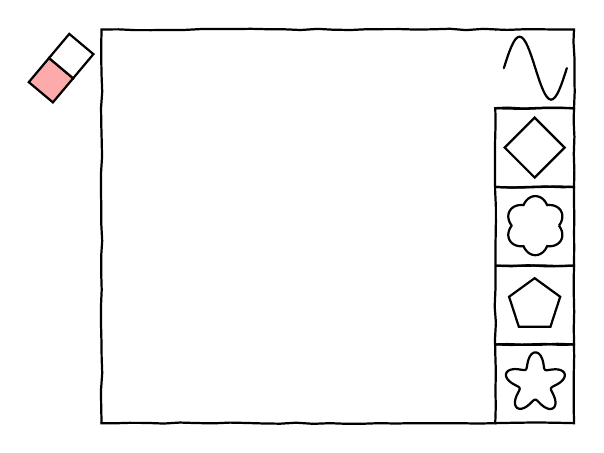
\begin{tikzpicture}[
	decoration={random steps,segment length=6pt,amplitude=0.25pt},
	thick
]

	% definitions
	\def\w{5}
	\def\n{5}
	\def\p{4}
	\pgfmathsetmacro{\nMinusOne}{int(\n-1)}
	\pgfmathsetmacro{\pPlusOne}{int(\p+1)}
	\pgfmathsetmacro{\nInverse}{\w/\n}
	\pgfmathsetmacro{\eraserScale}{.08*\w}
	
	\begin{scope}[local bounding box=scope1]

	% define nodes
	\coordinate[outer sep=0pt] (00) at (0,0) {};	
	\coordinate (10) at (\w,0) {};	
	\coordinate (11) at (\w,\w) {};	
	\coordinate (01) at (0,\w) {};
	
	\foreach \i in {0,...,\n}{
		\coordinate (\i) at (\w,\nInverse*\i) {};
		\coordinate (\i+) at (\w+\nInverse,\nInverse*\i) {};
	}
	
	% draw outlines
	\draw[decorate] (00) -- (01) -- (11) -- ([yshift=-.5\pgflinewidth]\pPlusOne);
	\draw[decorate] ([yshift=.5\pgflinewidth]\p) -- (10) -- ([xshift=-.5\pgflinewidth]00);
	
	\foreach \i in {0,...,\nMinusOne}{
		\pgfmathsetmacro{\iPlusOne}{int(\i+1)}
		\draw[decorate] (\i) -- (\i+) -- (\iPlusOne+) -- (\iPlusOne);
	}
	
	\end{scope}
	
	% eraser
	\begin{scope}[shift={($(scope1.north west)+(-\nInverse/2,-\nInverse/2)$)},rotate=50]
		\begin{scope}[scale=\eraserScale]
			\draw[fill=pink] (-1,-0.5) --++ (1,0) --++ (0,1) --++ (-1,0) -- cycle;
			\draw[fill=white] (0,-0.5) --++ (1,0) --++ (0,1) --++ (-1,0) -- cycle;
		\end{scope}
	\end{scope}
	
	% free draw
	\begin{scope}[shift={($(scope1.north east)+(-\nInverse/2,-\nInverse/2)$)}]
		\begin{scope}[scale=\nInverse/5]
			\draw[line cap=round] (-2,0) sin (-1,2) cos (0,0) sin (1,-2) cos (2,0);
		\end{scope}
	\end{scope}
	
	% diamond
	\def\p{3}
	\node[scale=\w/3,draw,diamond] at (\w+\nInverse/2,\p*\nInverse+\nInverse/2) {};
	
	% flower
	\def\p{2}
	\begin{scope}[shift={($(scope1.north east)+(-\nInverse/2,-\p*\nInverse-\nInverse/2)$)}]
		\begin{scope}[scale=\nInverse/5]
			\draw[domain=0:360,scale=1.5,samples=500] plot ({\x}:{1+.25*abs(sin(3*\x))});
		\end{scope}
	\end{scope}
	
	% pentagon
	\def\p{1}
	\node[scale=\w/3,draw,regular polygon,regular polygon sides=5] at (\w+\nInverse/2,\p*\nInverse+\nInverse/2) {};
	
	% star
	\def\p{4}
	\begin{scope}[shift={($(scope1.north east)+(-\nInverse/2,-\p*\nInverse-\nInverse/2)$)}]
		\begin{scope}[scale=\nInverse/5]
			\draw[domain=0:360,scale=1.5,samples=500] plot ({\x}:{abs(1+0.3*sin(5*\x+pi/2))});
		\end{scope}
	\end{scope}
	
	

            
	
\end{tikzpicture}

\end{document}